% Options for packages loaded elsewhere
\PassOptionsToPackage{unicode}{hyperref}
\PassOptionsToPackage{hyphens}{url}
\PassOptionsToPackage{dvipsnames,svgnames,x11names}{xcolor}
%
\documentclass[
  letterpaper,
  DIV=11,
  numbers=noendperiod]{scrartcl}

\usepackage{amsmath,amssymb}
\usepackage{iftex}
\ifPDFTeX
  \usepackage[T1]{fontenc}
  \usepackage[utf8]{inputenc}
  \usepackage{textcomp} % provide euro and other symbols
\else % if luatex or xetex
  \usepackage{unicode-math}
  \defaultfontfeatures{Scale=MatchLowercase}
  \defaultfontfeatures[\rmfamily]{Ligatures=TeX,Scale=1}
\fi
\usepackage{lmodern}
\ifPDFTeX\else  
    % xetex/luatex font selection
\fi
% Use upquote if available, for straight quotes in verbatim environments
\IfFileExists{upquote.sty}{\usepackage{upquote}}{}
\IfFileExists{microtype.sty}{% use microtype if available
  \usepackage[]{microtype}
  \UseMicrotypeSet[protrusion]{basicmath} % disable protrusion for tt fonts
}{}
\makeatletter
\@ifundefined{KOMAClassName}{% if non-KOMA class
  \IfFileExists{parskip.sty}{%
    \usepackage{parskip}
  }{% else
    \setlength{\parindent}{0pt}
    \setlength{\parskip}{6pt plus 2pt minus 1pt}}
}{% if KOMA class
  \KOMAoptions{parskip=half}}
\makeatother
\usepackage{xcolor}
\setlength{\emergencystretch}{3em} % prevent overfull lines
\setcounter{secnumdepth}{-\maxdimen} % remove section numbering
% Make \paragraph and \subparagraph free-standing
\ifx\paragraph\undefined\else
  \let\oldparagraph\paragraph
  \renewcommand{\paragraph}[1]{\oldparagraph{#1}\mbox{}}
\fi
\ifx\subparagraph\undefined\else
  \let\oldsubparagraph\subparagraph
  \renewcommand{\subparagraph}[1]{\oldsubparagraph{#1}\mbox{}}
\fi


\providecommand{\tightlist}{%
  \setlength{\itemsep}{0pt}\setlength{\parskip}{0pt}}\usepackage{longtable,booktabs,array}
\usepackage{calc} % for calculating minipage widths
% Correct order of tables after \paragraph or \subparagraph
\usepackage{etoolbox}
\makeatletter
\patchcmd\longtable{\par}{\if@noskipsec\mbox{}\fi\par}{}{}
\makeatother
% Allow footnotes in longtable head/foot
\IfFileExists{footnotehyper.sty}{\usepackage{footnotehyper}}{\usepackage{footnote}}
\makesavenoteenv{longtable}
\usepackage{graphicx}
\makeatletter
\def\maxwidth{\ifdim\Gin@nat@width>\linewidth\linewidth\else\Gin@nat@width\fi}
\def\maxheight{\ifdim\Gin@nat@height>\textheight\textheight\else\Gin@nat@height\fi}
\makeatother
% Scale images if necessary, so that they will not overflow the page
% margins by default, and it is still possible to overwrite the defaults
% using explicit options in \includegraphics[width, height, ...]{}
\setkeys{Gin}{width=\maxwidth,height=\maxheight,keepaspectratio}
% Set default figure placement to htbp
\makeatletter
\def\fps@figure{htbp}
\makeatother

\KOMAoption{captions}{tableheading}
\makeatletter
\@ifpackageloaded{caption}{}{\usepackage{caption}}
\AtBeginDocument{%
\ifdefined\contentsname
  \renewcommand*\contentsname{Table of contents}
\else
  \newcommand\contentsname{Table of contents}
\fi
\ifdefined\listfigurename
  \renewcommand*\listfigurename{List of Figures}
\else
  \newcommand\listfigurename{List of Figures}
\fi
\ifdefined\listtablename
  \renewcommand*\listtablename{List of Tables}
\else
  \newcommand\listtablename{List of Tables}
\fi
\ifdefined\figurename
  \renewcommand*\figurename{Figure}
\else
  \newcommand\figurename{Figure}
\fi
\ifdefined\tablename
  \renewcommand*\tablename{Table}
\else
  \newcommand\tablename{Table}
\fi
}
\@ifpackageloaded{float}{}{\usepackage{float}}
\floatstyle{ruled}
\@ifundefined{c@chapter}{\newfloat{codelisting}{h}{lop}}{\newfloat{codelisting}{h}{lop}[chapter]}
\floatname{codelisting}{Listing}
\newcommand*\listoflistings{\listof{codelisting}{List of Listings}}
\makeatother
\makeatletter
\makeatother
\makeatletter
\@ifpackageloaded{caption}{}{\usepackage{caption}}
\@ifpackageloaded{subcaption}{}{\usepackage{subcaption}}
\makeatother
\ifLuaTeX
  \usepackage{selnolig}  % disable illegal ligatures
\fi
\usepackage{bookmark}

\IfFileExists{xurl.sty}{\usepackage{xurl}}{} % add URL line breaks if available
\urlstyle{same} % disable monospaced font for URLs
\hypersetup{
  pdftitle={Spatial Dynamics of Sweetgreen and Chipotle Locations: Proximity or Competition?},
  colorlinks=true,
  linkcolor={blue},
  filecolor={Maroon},
  citecolor={Blue},
  urlcolor={Blue},
  pdfcreator={LaTeX via pandoc}}

\title{Spatial Dynamics of Sweetgreen and Chipotle Locations: Proximity
or Competition?}
\usepackage{etoolbox}
\makeatletter
\providecommand{\subtitle}[1]{% add subtitle to \maketitle
  \apptocmd{\@title}{\par {\large #1 \par}}{}{}
}
\makeatother
\subtitle{DSAN 6750 / PPOL 6805: GIS for Spatial Data Science}
\author{Bella Shi \and Jacky Zhang \and Lianghui Yi}
\date{}

\begin{document}
\maketitle

\subsection{Introduction}\label{introduction}

This project investigates whether the spatial distributions of
Sweetgreen and Chipotle locations in the United States are correlated.
We test if the chains cluster together (suggesting direct competition)
or show patterns of spatial repulsion. Our hypothesis is:

\begin{itemize}
\item
  \(\mathcal{H}_0\): Sweetgreen and Chipotle locations are randomly
  distributed with no spatial correlation.
\item
  \(\mathcal{H}_A\): Sweetgreen and Chipotle locations are spatially
  correlated (either clustering or repelling).
\end{itemize}

\subsection{Methodology}\label{methodology}

We employ spatial analysis tools and a Monte Carlo simulation to assess
spatial correlation. Using a spatial lag model and randomization tests,
we compare observed distances between Sweetgreen and Chipotle locations
with a distribution of distances under randomized placement of Chipotle
locations.

Key Steps:

\begin{verbatim}
1.  Data Collection & Geocoding: Using the Google Places API to gather restaurant coordinates.
2.  Exploratory Data Analysis: Mapping and visualizing the distributions.
3.  Monte Carlo Simulation: Testing whether observed proximity differs from random expectations.
4.  Statistical Tests: Conducting a one-sample t-test on the simulated distribution to determine significance.
\end{verbatim}

\subsection{Collecting Data}\label{collecting-data}

Below is an example snippet showing how we used the Google Places API to
collect locations. We save outputs in GeoJSON, GeoPackage, and Shapefile
formats. (Actual API keys and code omitted for brevity.)

\phantomsection\label{data_collection}
\begin{verbatim}
Fetched 18 places.
Saved GeoJSON to output/sweetgreen_locations_geojson_2024.geojson
Saved GeoPackage to output/sweetgreen_locations_geopackage_2024.gpkg
Saved Shapefile to output/sweetgreen_locations_shapefile_2024.shp
\end{verbatim}

\begin{verbatim}
Fetched 20 places.
Saved GeoJSON to output/chipotle_locations_geojson_2024.geojson
Saved GeoPackage to output/chipotle_locations_geopackage_2024.gpkg
Saved Shapefile to output/chipotle_locations_shapefile_2024.shp
\end{verbatim}

\subsection{Preprocessing Data}\label{preprocessing-data}

\subsection{Exploratory Data Analysis
(EDA)}\label{exploratory-data-analysis-eda}

After collecting data, we geocode and plot the locations. We create
intensity maps and heatmaps to visually inspect spatial patterns.

\subsubsection{Intensity Map of Sweetgreen and Chipotle
Locations}\label{intensity-map-of-sweetgreen-and-chipotle-locations}

\begin{verbatim}
<folium.folium.Map at 0x16a297350>
\end{verbatim}

\subsubsection{Heatmap of Sweetgreen and Chipotle
Locations}\label{heatmap-of-sweetgreen-and-chipotle-locations}

\begin{verbatim}
<folium.folium.Map at 0x16911f290>
\end{verbatim}

\subsection{Hypothesis}\label{hypothesis}

\subsubsection{Hypothesis:}\label{hypothesis-1}

\(\mathcal{H}_0\): Sweetgreen and Chipotle locations are randomly
distributed with no spatial correlation.

\(\mathcal{H}_A\): SSweetgreen and Chipotle locations are spatially
correlated (either clustering together (proximity) or repelling each
other (competition)).

\subsubsection{Monte Carlo Simulation}\label{monte-carlo-simulation}

To test our hypothesis, we conduct a Monte Carlo simulation. We randomly
distribute Sweetgreen and Chipotle locations on a map and calculate the
distance between each pair of locations. We then compare the observed
distance between Sweetgreen and Chipotle locations to the distribution
of distances under the null hypothesis.

Steps:

\begin{enumerate}
\def\labelenumi{\arabic{enumi}.}
\tightlist
\item
  Calculate observed distances between Sweetgreen and Chipotle using the
  minimum distance to a Chipotle for each Sweetgreen location.
\item
  Randomize Chipotle locations within the bounding box
  (longitude-latitude range of original Chipotle locations).
\item
  Repeat this process for the specified number of simulations, storing
  the average distance for each simulation.
\end{enumerate}

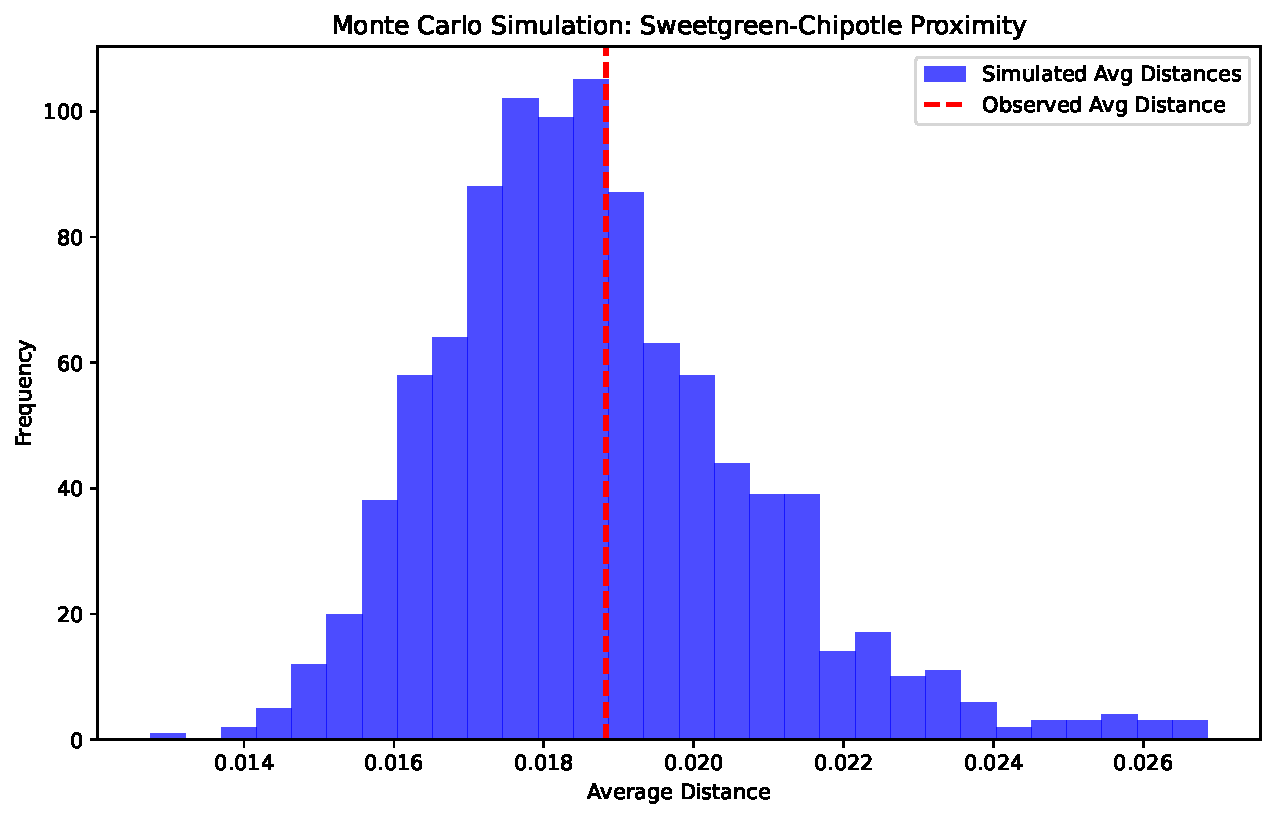
\includegraphics{index_files/figure-pdf/cell-7-output-1.pdf}

\subsubsection{KDE Plot of Sweetgreen and Chipotle
Locations}\label{kde-plot-of-sweetgreen-and-chipotle-locations}

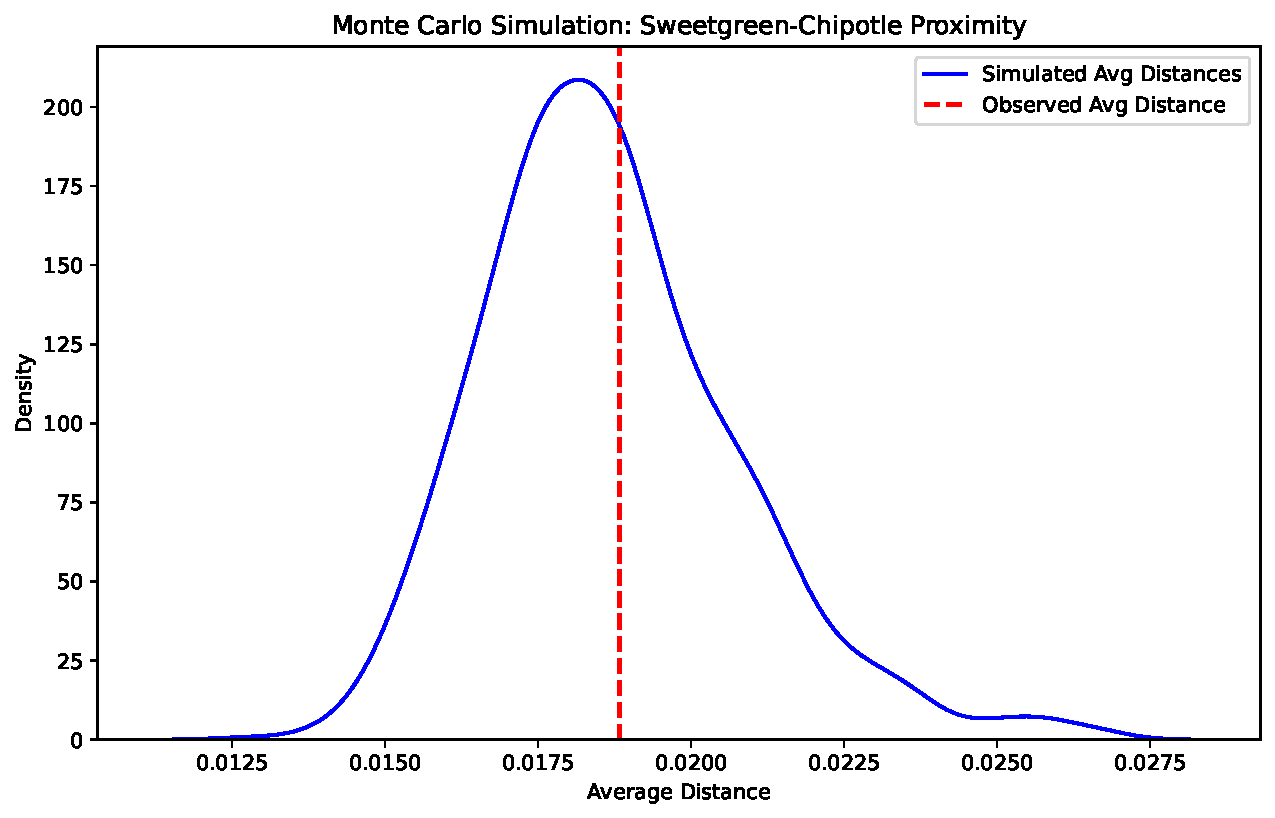
\includegraphics{index_files/figure-pdf/cell-8-output-2.pdf}

\begin{verbatim}
The observed average distance is not significantly shorter. This suggests they are not spatial corralated.
\end{verbatim}

\paragraph{One-Sample T-Test}\label{one-sample-t-test}

Hypothesis:

\(\mathcal{H}_0\): Sweetgreen and Chipotle locations are randomly
distributed with no spatial correlation.

\(\mathcal{H}_A\): Sweetgreen and Chipotle locations are spatially
correlated (either clustering together (proximity) or repelling each
other (competition).

\begin{verbatim}
T-statistic: -2.3336760738297295
P-value: 0.01981027122504727
The observed average distance is significantly different from the simulated distances (reject H₀).
\end{verbatim}

\subsection{Discussion}\label{discussion}

If the locations of Sweetgreen and Chipotle are spatially correlated,
Are Sweetgreen and Chipotle locations clustered together (like in the
Hotelling model)? Or are they evenly spaced across a city or region
(like in the Salop model)?

\subsubsection{1. Hotelling Model (Linear City
Model)}\label{hotelling-model-linear-city-model}

Concept: Firms compete for customers along a single line (like a street,
highway, or product spectrum). Customers are evenly distributed along
the line and face ``transportation costs'' (effort, time, or money) to
reach the firms.

Firms tend to move closer together toward the center of the line
(``minimum differentiation'') to capture the largest customer base. This
``clustering'' happens because if one firm moves away, it loses
customers to its competitor. Application to Sweetgreen vs.~Chipotle: We
can use the Hotelling model to analyze whether these two chains are
colocated (clustered) to maximize competition or spread out to dominate
separate areas. The average distances between Sweetgreen and Chipotle
locations serve as a proxy for their competitive strategy.

\subsubsection{2. Salop Model (Circular City
Model)}\label{salop-model-circular-city-model}

Concept: Extends the Hotelling model to a circular city (like a city
with multiple neighborhoodsor a ring road). The circular model is useful
when more than two competitors exist, and it prevents boundary effects
(e.g., firms clustering at the ends of a line).

Goal: Firms aim to maximize market share by minimizing transportation
costs for customers, similar to the Hotelling model, but in a circular
(2D) representation.

Customers are evenly distributed around a circle. Multiple firms (e.g.,
Sweetgreen, Chipotle, Panera Bread) compete. Customers pick the closest
firm, incurring the lowest transportation cost. Implications: Firms tend
to space themselves equally around the circle to avoid direct
competition and capture their segment of the market. This leads to
``maximum differentiation,'' where firms spread out rather than cluster
together.

Salop's Model assumes businesses (like Sweetgreen and Chipotle) are
evenly distributed on a circular market, leading to relatively
equidistant placements. A low standard deviation in the closest
distances ( min\_distances min\_distances) would be consistent with this
model, as it reflects uniform proximity to competitors.

\begin{verbatim}
Standard Deviation of Min Distances: 0.0234
High standard deviation in distances suggests clustering or irregular spacing, not consistent with Salop's Model.
\end{verbatim}

\subsubsection{3. Hotelling Model: Analyze Minimum
Distances}\label{hotelling-model-analyze-minimum-distances}

We compute the average minimum distance from each Sweetgreen to the
nearest Chipotle to assess clustering.

\begin{verbatim}
Average minimum distance between Sweetgreen and Chipotle: 0.01 miles
\end{verbatim}

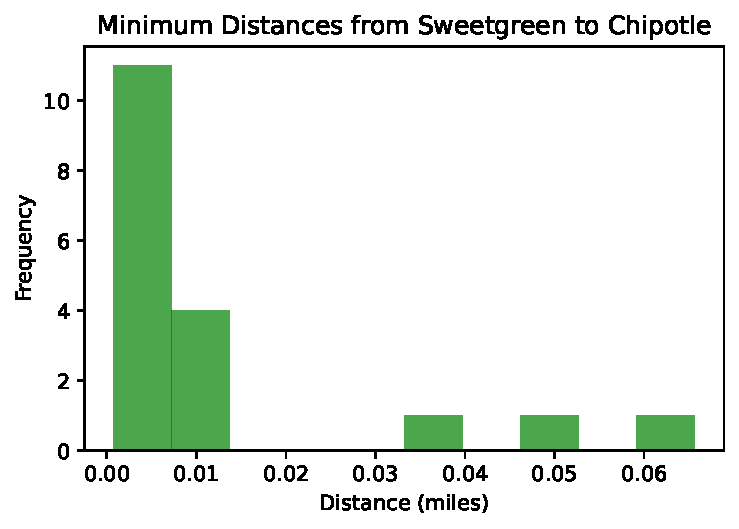
\includegraphics{index_files/figure-pdf/cell-11-output-2.pdf}

Use minimum distances between Sweetgreen and Chipotle to assess
clustering or separation.

A smaller average distance indicates clustering (competitive strategy).

\subsubsection{4. Salop Model: Voronoi Diagram for Market
Coverage}\label{salop-model-voronoi-diagram-for-market-coverage}

We compute the Voronoi diagram to visualize how Sweetgreen and Chipotle
locations partition space and analyze their spatial distribution.

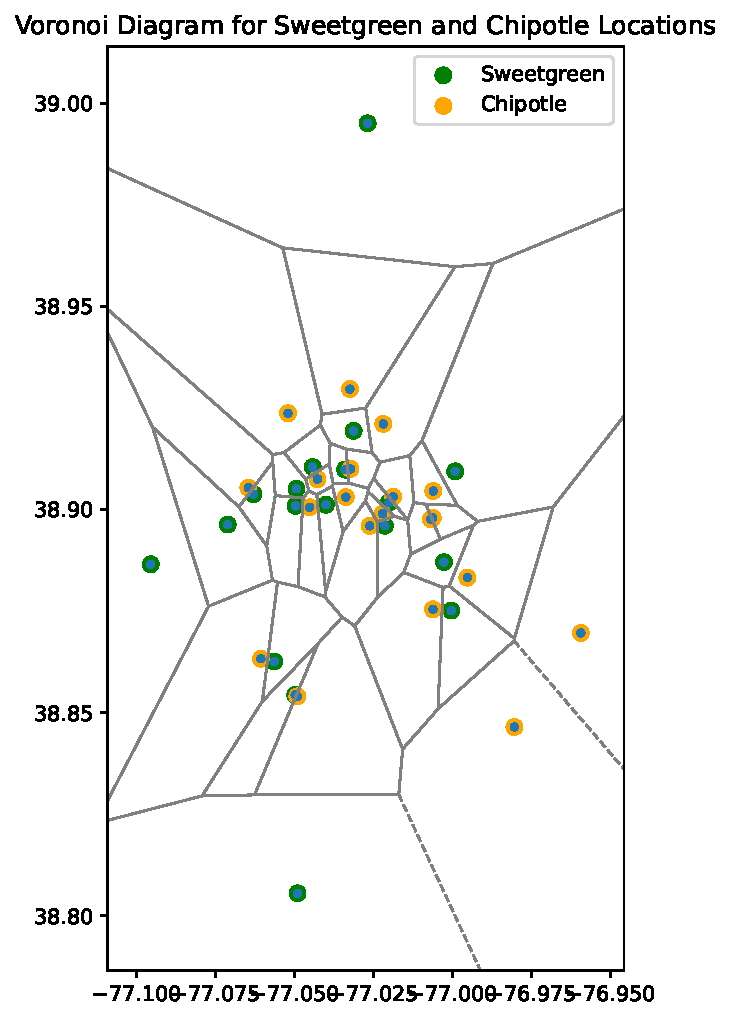
\includegraphics{index_files/figure-pdf/cell-12-output-1.pdf}

Use Voronoi diagrams to assess market partitioning and spatial
competition. Equal partitioning suggests maximum differentiation, while
overlap indicates clustering.

\subsection{Conclusion}\label{conclusion}

Sweetgreen and Chipotle are not randomly distributed. Their locations
exhibit spatial correlation, indicating strategic positioning.
Policymakers and businesses should consider these patterns when shaping
food environments, as they may influence consumer choices and community
health outcomes.



\end{document}
